\section{\revision{Joining the Strands in AdaCAD}}
\label{ch_adacad}

\revision{The strands of digital fabrication, textiles, and social justice began converging at the start of my PhD studies. 
% My research in e-textiles would not be possible without foundational work from these three domains discussed above: HCI, textiles, and social justice. What does synthesizing all of these topics look like? 
In my first year, I joined the Unstable Design Lab to help develop AdaCAD, open-source software for designing woven e-textiles. 
% To conclude this background chapter, I will briefly recount my own introduction to this interdisciplinary space. 
This section recounts this initial project, which went on to serve as a foundation for my later projects. Practically, AdaCAD's codebase was the foundation for several software tools I created; conceptually and theoretically, AdaCAD's design was where retooling and coproduction took root as themes in my research.} 
% concluding with the present day where I develop these concepts' definitions in the context of e-textiles. 
I aim to retroactively capture unconscious threads in my practice: that I kept engaging with tools, thinking about weaving, and trying to foreground sustainability and intersectional environmentalism as an important cause for technological development. In the context of the literature review, I argue that this research narrative demonstrates the motivating effectiveness of the retooling and coproduction for e-textiles design.

\subsection{Integrating Craft into Technical Practice }

\revision{AdaCAD's development was led by} fellow first-year Mikhaila Friske, also advised by Laura Devendorf. AdaCAD was to be a computer-aided design (CAD) software tool for designing woven e-textiles. The project was motivated by a lack of such tools that supported specific needs of the practice, notably designing both woven structures and electronic circuits simultaneously. As a first-year project, AdaCAD was my introduction to weaving, smart textiles, and HCI research in computational design tools. It also was my introduction to the concept of ``coproduction'', challenging me to examine two formerly-separate skillsets (yarn crafts and electronic hardware) as one entangled knowledge system.

\begin{figure}
  \centering
  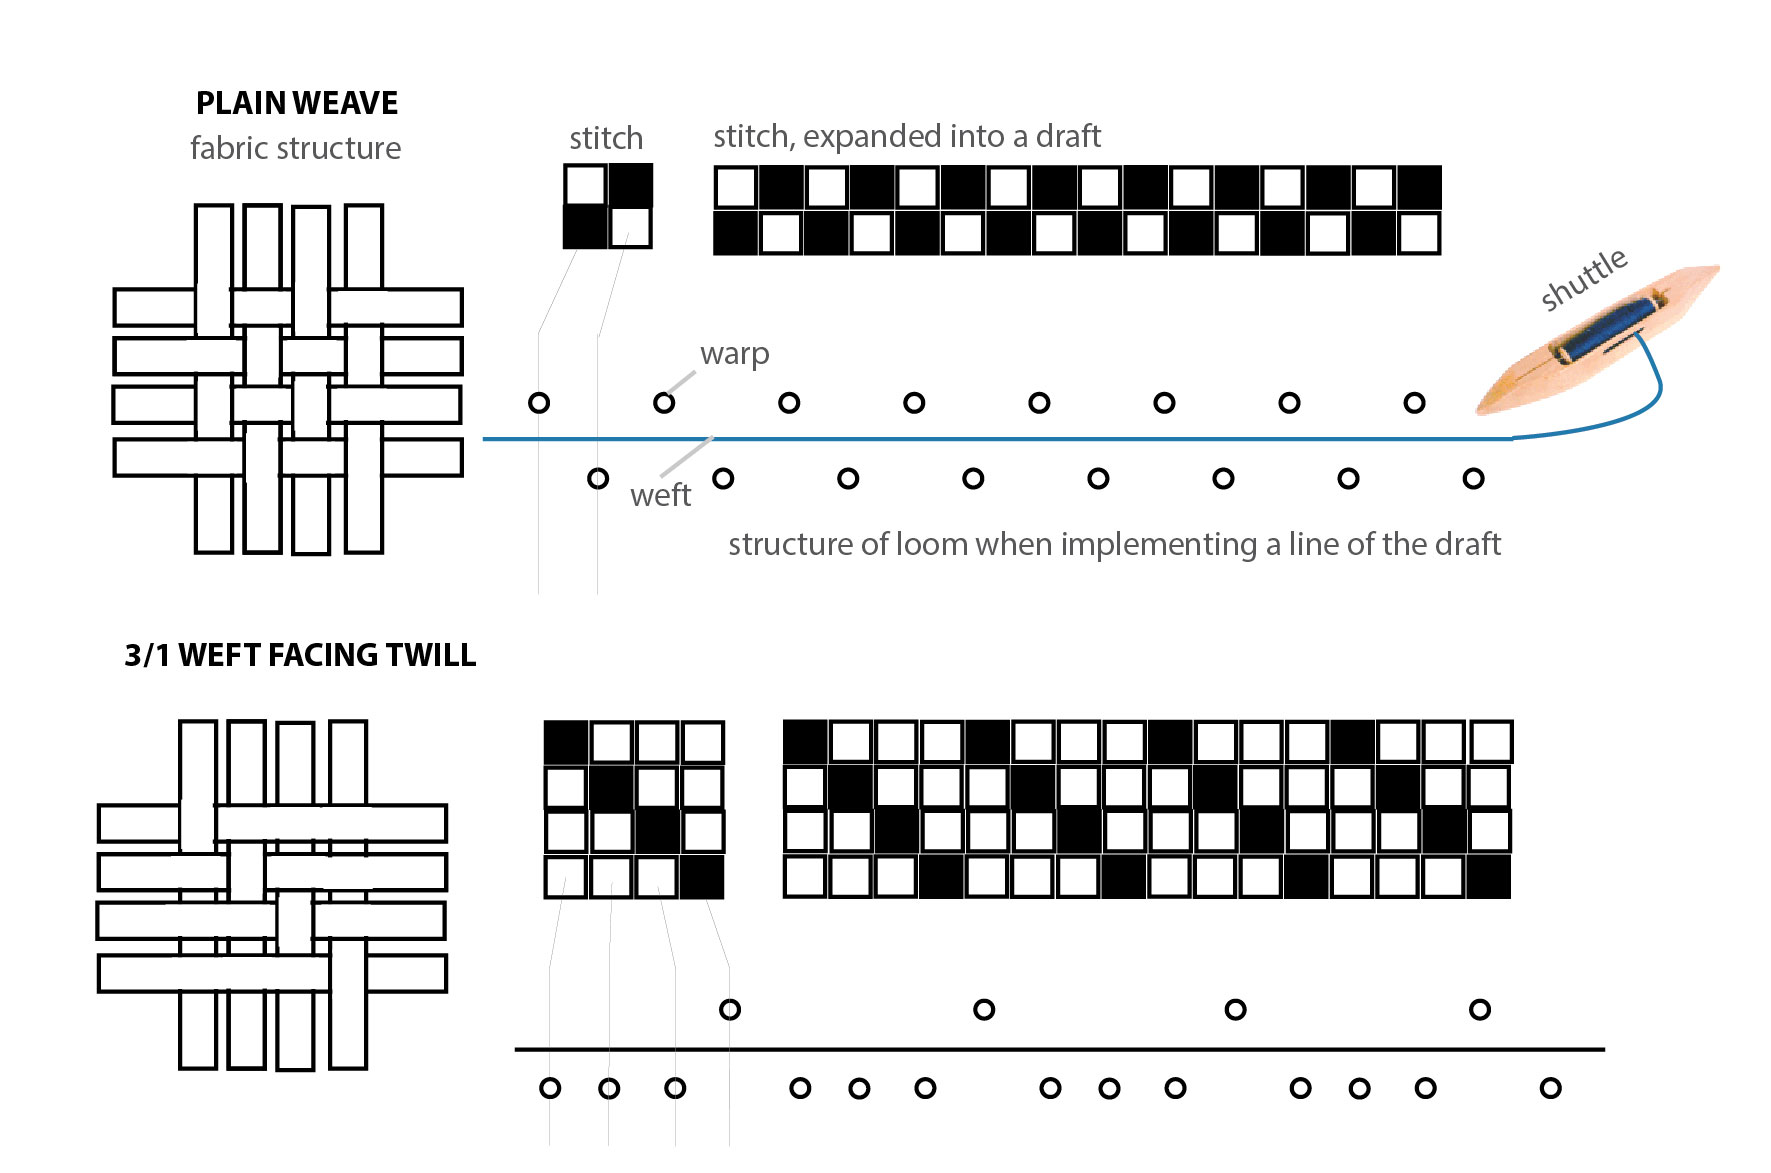
\includegraphics[width=0.6\textwidth]{figs/AdaCAD_weavedrafts_300.jpg}
  \caption[Examples of weaving draft notation.]{Descriptions of how a weave draft represents a woven structures and how a loom implements those drafts to create those structures.
  }
  \label{fig:adacad-drafts}
\end{figure}

My part on the project started at a week-long workshop at the Jacquard Center in Hendersonville, North Carolina, where I learned how to weave on a TC2 digital Jacquard loom for the first time --- or for that matter, any loom that was more mechanically complex than a tapestry loom. I also learned how to use Adobe Photoshop to create drafts, or design files, for the TC2, which is one of the most widely-used software tools among TC2 weavers. Conceptually, I started to understand how the draft is a data format for looms, how a loom processes this data and thus performs computation, and where a conventional digital computer could be placed in this workflow (see Fig. \ref{fig:adacad-drafts}). AdaCAD represented how coproduction could trouble default technological narratives and not only make a designer aware of conventional computing's privilege over textiles, but also challenge them to subvert this dynamic.

\subsection{Retooling Textiles Craft in Software}

Even during this single week, with my weaving practice in its infancy, I began to appreciate weaving as a computational domain with compelling challenges. I fixated on double weaving, a category of woven structures where two layers of cloth are woven simultaneously. From my experiences in the workshop, I was able to provide Mikhaila and Laura with my first impressions of woven design on the TC2, and observations of common techniques and challenges as shared by the instructor, Cathryn Amidei, and my fellow workshop participants. These reflections informed Mikhaila as they implemented AdaCAD's key features in code. Meanwhile, Laura had also been perplexed by double weaving because the basic structure's draft representation did not intuitively map to the physical cloth.

% The paper, as submitted at the end of 2018, describes the process and development of the first version of AdaCAD (UI overview in Fig. 2), an application for composing smart textile weave drafts. By augmenting traditional weaving drafts, AdaCAD allows weavers to design woven structures and circuitry in tandem and offers specific support for common smart textiles techniques. We describe these techniques, how our tool supports them alongside feedback from smart textiles weavers. We conclude with a reflection on smart textiles practice more broadly, and suggest that the metaphor of coproduction can be fruitful in creating effective tools and envisioning future applications in this space.
Our collective experiences helped us understand, from a conceptual and embodied perspective, where design tools could be most effective in supporting e-textiles development. Through the process, four key principles emerged:

\begin{enumerate}
\item Prioritize drafts over simulation.
\item Explicitly support textiles techniques.
\item The software must help the user understand yarn paths within the fabric.
\item Designers should learn from weaving software (rather than PCB software or other electronics CAD).
\end{enumerate}

Because all of these principles prioritized the ``textiles'' in smart textiles design such as following yarn paths rather than circuit traces, I came to understand that coproduction, by troubling existing technological narratives such as ``hybrid'' and which technologies were considered ``smart'' or were recognized for their computational capacity, could aid in subverting the privileging of conventional computing over textiles in such a domain. AdaCAD's creation represented a way to put modern computing in service to textiles. I was particularly struck at the revelation that weaving software would be more informative for our design than electronic CAD, as from my physics background, I was still unlearning the constructed hierarchies between ``high-tech'' digital devices and ``low-tech'' textiles, all of which I was beginning to understand as forms of computing.

Retooling, as my entry point into an unfamiliar design domain, forced me to quickly acquaint myself with existing tools used by smart textiles practitioners and their guiding design principles. For one, I learned how weaving, from simple tapestries to fully-automated industrial wovens, operated on a data format (drafts) that could be easily translated across representations (paper vs. bitmap files) and re-interpreted for many different types of loom machinery. In contrast, the circuit schematics which I was familiar with often required specialized symbols to render, and would still lose spatial fidelity by representing the circuit's electrical functions. While traditional drafts do convey structural as well as functional information, AdaCAD showed the importance of having several ``views'' into a multi-dimensional design such as a woven smart textile. 
% AdaCAD offers two view options for the user while creating the weave draft: yarn view and pattern view. The pattern view is used to design the draft itself, while the yarn view shows the path of each continuous piece of yarn. Thus, the pattern view shows the traditional weave information while the yarn view shows a schematic view like one might see in Eagle or Fritzing. The primary purpose of the yarn view is to aid in visualizing the connectivity of the circuit components: the yarn view helps a smart textiles weaver assess whether or not their yarns are going to cross or short; it offers insight into how the human ought to execute the pattern by showing them, for instance, whether or not they should pass the shuttle into the weave on the left or right side to achieve their desired structure; And lastly, the yarn view includes labels on the ends of the yarn path for planning connections to elements like PCBs and microcontrollers.
\revision{To follow Jennifer Jacobs' suggestion} that linked views in CAD tools support viewing the design through multiple lenses \cite{jacobs_codeable_2013}. In our case with AdaCAD, these lenses are those of a weaver and a circuit designer. 

Retooling my view on craft practices as technological innovation, I came to realize how a crafter such as a e-textiles weaver holds several positions in realizing their design, that would each be a separate role were this a traditional embedded development project: mechanical engineer, electrical engineer, system architect, as well as textile design and fabrication. AdaCAD's key features deconstructed my existing assumptions about how a design tool needed to be optimized for a particular task or role, giving language to my subconscious love of how craft processes embodied the artifact's whole life and retooling my notions of what design software could support in people's practices.

\subsection{Artifacts of Coproduction}

In creating several woven smart textiles while working on AdaCAD with my colleagues, I gained additional examples of how smart textiles artifacts were coproductions of textiles and electronics practices, including the involved materials and structures. As a retool, AdaCAD's design was in response to the influences of these and other tools in the practice, including Photoshop as I had learned to use it at the Jacquard Center as well as paper notation systems still used by many weavers \cite{chandler_learning_2009}. But also as a coproduction of these tools, AdaCAD did not simply ``hybridize'' their different features, but actively questioned what these features represented in their respective textile and electronic artifacts and whether they were truly distinct structures and practices at all. 
% In the original paper, we presented the following examples in order of ``complexity", which I have re-ordered somewhat to instead highlight components versus assemblages that form a gestalt whole. 

% Figure 3 shows how AdaCAD could be used to design a double-woven fabric to act as a press button. It also recalls how perplexed we were all by doubleweaving in the process of developing AdaCAD, that the woven structure was present in many of the prototypes we wove to test AdaCAD's capabilities and that it posed an edge case to several features. This first example (which I did not weave) demonstrates a common technique in smart textiles that creates press buttons by leveraging the 2-layer structure of double weaving [16]: a coproduct of woven and electromechanical structures.

\begin{figure}[h]
  \centering
  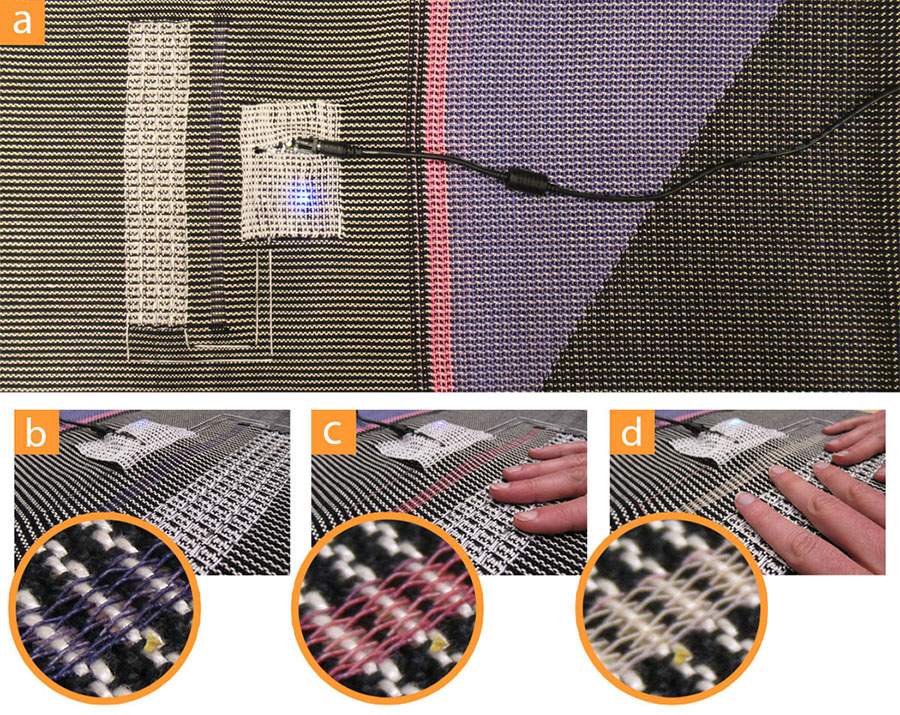
\includegraphics[width=0.6\linewidth]{figs/AdaCAD_multicomp.jpg}
  \caption[A multi-component woven e-textile.]{Multi-Component woven smart textile, containing (a, left to right) waffle stitch pressure sensor, color changing strip, and pocket for PCB; (b) initial state before press; (c) pressure sensor state 1, color change to red/pink; (d) pressure sensor state 2, color change to white.
  }
  \label{fig:multicomp-weave}
\end{figure}

After being acquainted with Photoshop, I also began using AdaCAD to design drafts to help shape features which could better facilitate designing circuitry in a fabric. In another retool of my developing practice, I also learned how to use a more ``analog'' or traditional floor loom while the lab was awaiting the TC2's delivery. 
% Another technique with which the lab was actively experimenting was dyeing yarns with thermochromic pigments, which would change color when exposed to different temperatures, such as resistive heating from a conductive yarn. AdaCAD's different views, along with the ``image import'' feature that Mikhaila added, gave me a tool to design overlapping color-changing regions in the Interwoven Images fabric, thus creating multi-state smart textile actuation or display (Fig. 4). The greatest challenge in this design was not the circuitry, as each color-changing region was simply a single wire wrapped in cotton and colored with thermochromic. Rather, the woven structure itself was integral to achieving the electrical function, as the regions had to be thermally isolated from each other by the non-conductive cotton yarns, even though they were overlapping visually. 
% In retrospect, this piece is a coproduct of my learning processes in electronics and computing systems prior to weaving, with my textiles knowledge of yarn crafts that had begun in knitting and crochet. The textile circuit's physical layout was the result of a choreography of shuttles carrying the different yarns, conductive color-changing and insulating cotton, in the plane of the fabric (back and forth, from bottom to top), as well above and below the fabric's plane.

As my sense of coproduction between the different knowledge domains grew, I was better able to synthesize textiles and electronics into a cohesive system. The next weaving I produced, the Multi-component Weave, aimed to implement a complete input-output (I/O) system in the fabric, consisting of a pressure-sensor that would activate a color-changing region (Fig. \ref{fig:multicomp-weave}). Using a waffle weave structure and conductive yarn to create a pressure-sensing region, following KOBAKANT's documentation of the technique \cite{satomi_woven_2015}, I isolated the structure to only partially span the fabric's width. I used a similar technique as the Interwoven Images to weave a color-changing region with thermochromic yarn. Lastly, came the challenge of creating a housing for the Arduino microprocessor which would handle the I/O. Using my understanding of doubleweaving from the Jacquard Center, I fashioned a tunnel or pocket that was open at both sides, along with a slit in the top fabric to allow for the Arduino's plug. As a newer weaver, my workflow was largely improvised, leading me to switch between AdaCAD, paper notes, and the loom haphazardly. I actually found the foot-powered floor loom to be more efficient than the TC2 for experimenting with structures as I did with the different functional regions and the shaped pocket, as iterating my design was faster without having to create a new draft file every trial. Rather than creating a draft of the whole fabric before weaving, I created several smaller drafts to record the structural units for each section, which I then ``compiled'' into the larger draft after I was satisfied with the fabric. Looking back, this flexibility in my toolset offers an example of how a beginner's mindset in craft may be naturally open to retooling for coproduction, as the ``beginner'' designer has not yet strongly internalized values and techniques in the practice that a more experienced designer would.

Towards the end of development that summer, Laura led Mikhaila and I through a series of semi-structured interviews with other smart textiles (or smart textiles affiliated, if they did not consider themselves as part of ``textiles") practitioners who gave feedback on the working software prototype. Seeing their reactions to AdaCAD's features, along with Laura's and Mikhaila's explanations of how they had used those features, cemented that AdaCAD's coproduction was not only epistemological, but social as well, directly influenced by the needs of a wider community. 
% As a summative example of AdaCAD's features, I look again to another weaving that I did not make, but approached as a critical viewer and witness to its process.

% The Doubleweave multi-region fabric (Fig. 6) was woven earlier that summer, and an external electronic module to control the fabric's pressure sensing and heat-based color change was also developed in conjunction. This sample represents all of the weaving techniques I have discussed thus far (double-weaving, multi-functional yarns) along with my then ``traditional'' electronics knowledge of designing a circuit to put on a rigid board.

After that summer of initial development, AdaCAD has continued to evolve, along with my weaving practice, other tools in the lab, and the lab's research community. While I moved away from AdaCAD as my main project in subsequent years, the software became a reference point for how I could incorporate software tools into craft practices. By introducing ``coproduction'' into my design practice's vocabulary, the project gave me language to cherish my learning process as a beginner weaver, and name and honor my coproducing agents. Since that first year, I have always referred to the loom(s) I wove with as collaborators on a woven piece, as the weaving was also shaped by their machine specifics and differing design traditions. Although I would not recognize ``retooling'' until later in my studies, being aware of coproductive dynamics allowed me to be more sensitive to how my tools carried histories that far preceded myself, and retool them with the intent to respect their other lives. 
